\documentclass[a4paper, 12pt, twoside, article]{memoir}
\synctex=1

\counterwithout{section}{chapter}

\usepackage[utf8x]{inputenc}
\usepackage[T1]{fontenc}
\usepackage[english]{babel}

\usepackage[pdftex]{graphicx}

\usepackage[activate={true,nocompatibility},final,tracking=true,kerning=true,spacing=true,factor=1100,stretch=10,shrink=10,verbose=silent]{microtype}

\captiontitlefont{\itshape}
\usepackage[top=1in,bottom=1in,left=1.2in,right=1.2in]{geometry}

% Smaller spacing between lists
\usepackage{enumitem}
\setlist[itemize]{noitemsep}
\setlist[enumerate]{noitemsep}

\usepackage{cleveref}
\usepackage{minted}
\usepackage{hyperref}
\usepackage[nodayofweek]{datetime}

\title{Database Systems\\Mini Project}
%\date{\protect\formatdate{6}{2}{2014} to \protect\formatdate{6}{2}{2014}}
\date{\formatdate{6}{2}{2014}}
\author{
  Obeid, Elias\\
  \href{mailto:eobeid11@student.aau.dk}{\texttt{eobeid11@student.aau.dk}}
  \and
  Caspersen, Kent\\
  \href{mailto:kcaspe11@student.aau.dk}{\texttt{kcaspe11@student.aau.dk}}
  \and
  Madsen, Martin\\
  \href{mailto:mbma11@student.aau.dk}{\texttt{mbma11@student.aau.dk}}
}

\begin{document}

\frontmatter

\maketitle
\pagebreak

\mainmatter

\section{Self Study 1: Preliminary Database Modeling}
As stated in the assignment, we have decided to look at different possible attributes and models by looking at the structure of movie pages on IMDB\@. Initially, we think it would require many join tables, as we've identified a few many-to-many relationships among structures we've discussed. These structures are: \emph{actors}, \emph{directors}, \emph{writers}, \emph{movies}, \emph{awards}, \emph{ratings}, and \emph{users}.

\begin{figure}[H]
  \centering
  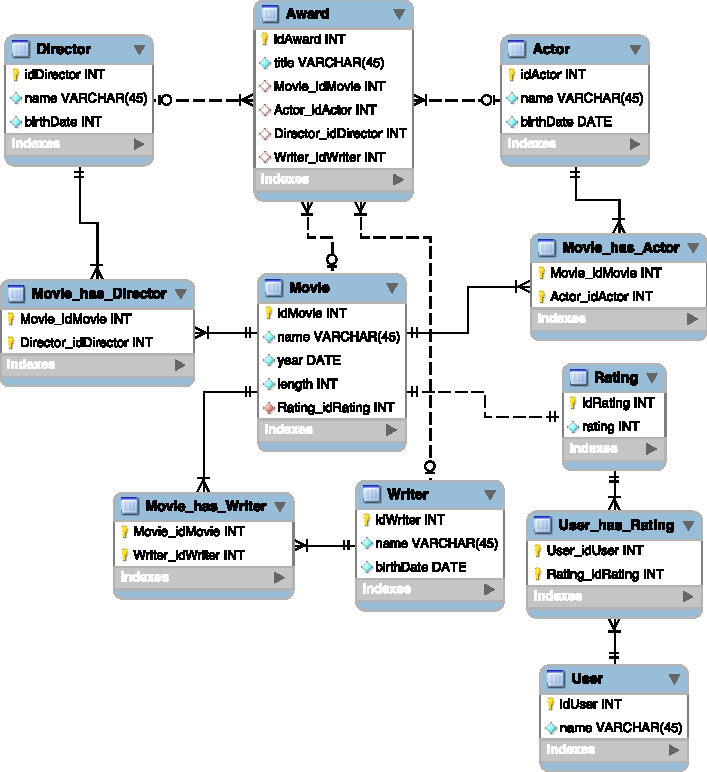
\includegraphics[width=\linewidth]{1-06.02.14/selfStudy1db.pdf}
  \caption{Enhanced entity-relationship (EER) model diagram of a simplified movie database.}\label{fig:model}
\end{figure}

The SQL for creating this structure, see \Cref{sec:sqlPre}.

\appendix

\chapter{SQL: Preliminary Database Modeling}\label{sec:sqlPre}
\inputminted{sql}{1-06.02.14/selfStudy1db.sql}

\end{document}
